%%%--------------------------------%%%
%%% Domain
%%%--------------------------------%%%

\section{Architecture}
\label{sec:DomainC}

In this chapter the used architectural patterns, technologies, frameworks and libraries are briefly explained. First, an overall composition is given whose individual layers will then be explicitly described.


\subsection{Overall composition}
\label{sec:DomainCa}
Based on the Model-View-Controller (\ac{MVC}) architectural pattern the application is split into three major parts: the frontend, backend and the persistence layer. As seen in figure \ref{fig:overallcomposition} the frontend is in charge of the view and the backend of the model and controller.

In terms of the \ac{MVC} pattern, the view / frontend is a presentational layer accessible by the user – traditionally a user interface. The model is equivalent to the data of an application which can be persisted with any appropriate technology (e.g. a database). The data itself can be accessed, updated or deleted by the controller. Furthermore, the controller is in charge of the logic of the application \cite[p. 7]{steyerWebanwendungenMitASP2017}.

\begin{figure}[h]
	\centering
	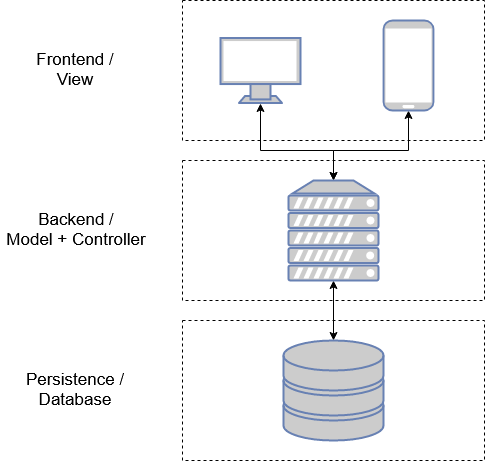
\includegraphics[width=0.6\textwidth]{Content/Domain/OverallComposition.png}
	\caption{Overall Composition}
	\cite{own representation}
	\label{fig:overallcomposition}
\end{figure}

\subsection{Frontend / View}
\label{sec:DomainCb}

The view of the application is primarly developed with React (Version 16.8.5, 19/11/2019) and Redux (Version 6.0.1, 19/11/2019).

React is a JavaScript library written by Facebook Inc. for developing user interfaces (typically web apps). The major benefits from using React are components and their states. Components (e.g. an alert) are written in \ac{JSX} and reusable which means when written once they can be reused anywhere else in the user interface, thus duplicate source code can be avoided. In React a component can hold its own state (e.g. the alert message or alert duration) which can be used for the user interface. If the state of a component changes and is involved in the user interface React automatically updates the user interface with the new state, making the development of the user interface easier as elements do not have to be addressed manually and then adjusted with the new content \cite[p. 7-8]{stefanovDurchstartenMitReact2017}.

Even though components can pass their states in hierarchical order, having a central store for the state of the components has several benefits as simplifying the overall project structure and easier testing. Redux is a JavaScript library providing such a store and introducing further terms described in the following list:

\begin{itemize}
	\item \textbf{Action}: An action typically leads to changes in the store but does not directly adjusts it. In fact, an action is responsible for fetching data from any resource (e.g. via the controller of the backend). The collected data will then be passed to a corresponding reducer.
	\item \textbf{Reducer}: A reducer contains the business logic about how exactly the data from the action should be saved to the store (e.g. filtering the action for only necessary information).
	\item \textbf{Store}: The store contains the state of the application and can be accessed by React components \cite[p. 531-534]{freemanProReact162019}. 
\end{itemize}

Figure \ref{fig:reduxpattern} visually explains the Redux pattern.

\begin{figure}[h]
	\centering
	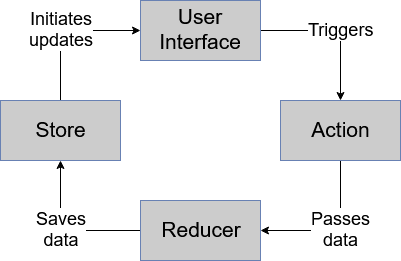
\includegraphics[width=0.6\textwidth]{Content/Domain/ReduxPattern.png}
	\caption{Redux Pattern}
	\cite{own representation}
	\label{fig:reduxpattern}
\end{figure}

\subsection{Backend / Model + Controller}
\label{sec:DomainCc}
The controller and model are mainly implemented with the help of Spring Boot 2 (Version 2.1.9, 20/11/2019) and the underlaying Spring Java framework (Version 5.1.10,  20/11/2019) developed by Pivotal Software. JHipster (Version 6.5.1, 20/11/2019), a tool for generating Spring Boot and React applications, is used for a fundamental setup.

The Spring Java framework is a popular framework to develop a variety of web applications with covering the needs for security and data persistence. As the needs of business applications are constantly growing, the Spring frameworks configuration became more complex \cite[p. 1]{prasadreddyBeginningSpringBoot2017}. With focus on extensibility and autoconfiguration Spring Boot was developed. The autoconfiguration is achieved by providing opinionated defaults whereas the extensibility is enabled by the possibility of adding starter modules such as Web, Data-\ac{JPA}  or Security \cite[p. 21-22]{prasadreddyBeginningSpringBoot2017}. 

All of them are used in the risk management application for the following purposes:

\begin{itemize}
	\item \textbf{Starter-Web}: This starter modules includes the Spring \ac{MVC} Java web framework providing support for the \ac{MVC} pattern and \ac{REST} \ac{API}s. For example, a Java class can be annotated as controller and methods within define what kind of \ac{HTTP} methods are allowed as well as the \ac{REST} endpoint the controller can be addressed at \cite[p. 107-109]{prasadreddyBeginningSpringBoot2017}. 
	\item \textbf{Starter-Data-\ac{JPA}}: The Starter-Data-JPA module allows developers to access databases in their Spring Boot application without writing \ac{SQL} statements. Instead an object oriented \ac{API} can be used and thus developers don’t have to switch between different languages. An important part of this module is Hibernate, a technology which can map Java objects to a database. Hence the whole model of the application can be realized as Java classes and the technologies in this starter module take care of the persistence to a database \cite[p. 83]{prasadreddyBeginningSpringBoot2017}. 
	\item \textbf{Starter-Security}: As not everyone should be able to access the same information or perform the same actions via the controllers (e.g. project related risks, deleting projects) the Starter-Security module enables security features such as authentication against the \ac{REST} endpoints or user specific roles like being an average user or application admin \cite[p. 176-176]{prasadreddyBeginningSpringBoot2017}. 
\end{itemize}

Figure \ref{fig:backenddetails} clarifies the functional interaction between all Spring Boot starter modules. In the case of the risk management application requests to \ac{REST} endpoints, implemented with features provided by the Starter-Web module, are performed by Redux actions (see chapter \ref{sec:DomainCb}). If the controller behind the \ac{REST} endpoint has restrictions to specific roles, specified with the help of the Starter-Security module, the roles are gathered from the user by the credentials which are sent with the request and if they match, the logic of the controller gets executed. In this example data should be retrieved which can be the gathered with the help of the object oriented JPA included in the Starter-Data-\ac{JPA} module and then be returned to the frontend and be used for further purposes. 

\begin{figure}[h]
	\centering
	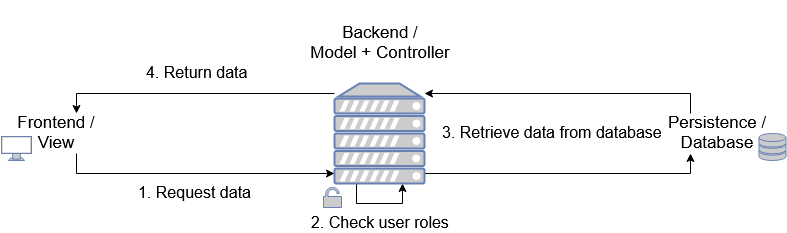
\includegraphics[width=1\textwidth]{Content/Domain/BackendDetails.png}
	\caption{Functional interaction of Spring Boot starter modules}
	\cite{own representation}
	\label{fig:backenddetails}
\end{figure}

\subsection{Persistence / Database}
\label{sec:DomainCd}

For persistence a relational PostgreSQL (Version 9.5, 20/11/2019) database is used and can be accessed by the backend. 

The creation of necessary tables and relations is being done automatically by the technologies within the Starter-Data-\ac{JPA} module. For further information about the Starter-Data-\ac{JPA} module see chapter \ref{sec:DomainCc}.

TODO: Add whole project UML here someday?

